%%
%% FloatLab (c) 2019-24 Christopher A. Bohn
%%
%% Assignment writeup licensed under the Creative Commons Attribution 4.0 International License
%% https://creativecommons.org/licenses/by/4.0/
%%

\documentclass[12pt]{article}

%%
%% labs/common/assignment.tex
%% (c) 2021-23 Christopher A. Bohn
%%
%% Licensed under the Apache License, Version 2.0 (the "License");
%% you may not use this file except in compliance with the License.
%% You may obtain a copy of the License at
%%     http://www.apache.org/licenses/LICENSE-2.0
%% Unless required by applicable law or agreed to in writing, software
%% distributed under the License is distributed on an "AS IS" BASIS,
%% WITHOUT WARRANTIES OR CONDITIONS OF ANY KIND, either express or implied.
%% See the License for the specific language governing permissions and
%% limitations under the License.
%%

\usepackage{addfont}
\usepackage{amsmath}
\usepackage{amssymb}
\usepackage{animate}
\usepackage{bold-extra}
\usepackage{cancel}
\usepackage{caption}
\usepackage{ccicons}
\usepackage{enumitem}
\usepackage{etoolbox}
\usepackage{fancyhdr}
\usepackage{fullpage}
\usepackage{graphicx}
\usepackage{hyperref}
\usepackage[utf8]{inputenc}
\usepackage[procnames]{listings}
%\usepackage{media9}
\usepackage{multicol}
\usepackage{subfig}
\usepackage{textcomp}
\usepackage{tikz}
\usepackage[americanresistor]{circuitikz}
\usepackage{tikz-uml}
\usetikzlibrary{automata,positioning,arrows}
\usepackage[normalem]{ulem}
\usepackage{wrapfig}
\usepackage{xcolor}
%\usepackage[dvipsnames]{xcolor}

\lstset{language=C, tabsize=4, upquote=true, basicstyle=\ttfamily}
\newcommand{\function}[1]{\textbf{\lstinline{#1}}}
\setlength{\headsep}{0.7cm}
\hypersetup{colorlinks=true}

%% CREDIT FOR MARKERLESSFOOTNOTE WHERE CREDIT IS DUE: https://tex.stackexchange.com/questions/30720/footnote-without-a-marker?answertab=scoredesc#tab-top
\newcommand\markerlessfootnote[1]{%
    \begingroup
    \renewcommand\thefootnote{}\footnote{#1}%
    \addtocounter{footnote}{-1}%
    \endgroup
}

\newcommand{\pagelayout}{
    \pagestyle{fancy}
    \fancyhf{}
    \lhead{\coursenumber}
    \chead{\ Lab \labnumber: \labname}
    \rhead{\courseterm}
    \cfoot{\shortlabname-\thepage}
}

\newcommand{\labidentifier}{
    \title{\ Lab \labnumber}
    \author{\labname}
    \date{Due: \duedate}
    \maketitle

    \textit{\collaborationrules}
    \markerlessfootnote{\tiny{\ifdefstring{\instructorname}{Christopher A. Bohn}{Assignment}{Original assignment} and starter code \copyright\ Christopher A. Bohn, licensed under the Creative Commons Attribution 4.0 International License~\ccby\ and under the Apache License Version 2.0, respectively.}}
    \ifdefstring{\instructorname}{Christopher A. Bohn}{}{\markerlessfootnote{\tiny{Configured for \coursenumber\ at \institutename\ by \instructorname.}}}

    \begin{description}
        \item[Obtaining the starter code] \filesource
        \item[Runtime environment] We will grade this assignment by compiling and running it on \runtimeenvironment;
            you should compile and test your code on \runtimeenvironment\ before turning it in.
        \item[Submitting your work] \filesubmission
    \end{description}
}

% display module fonts for hardware kit
% use with the Capital baseball "matrix printer" font collection (https://www.ctan.org/tex-archive/fonts/capbas/)
% Identifying the specific font in the assignment sheet is deprecated
%   -- instead, set the `usedisplayfont` boolean and the `displaymodule` variable in semester.tex,
%      and \display{...} in the assignment sheet

\addfont{OT1}{d7seg}{\dviiseg}
\addfont{OT1}{deseg}{\deseg}
\addfont{OT1}{necker}{\necker}

\providebool{usedisplayfont}

\newcommand{\display}[1]{
    \ifboolexpe{bool{usedisplayfont}}{
        \ifdefstring{\displaymodule}{MAX7219digits}{{\dviiseg #1}}{}
        \ifdefstring{\displaymodule}{MAX7219matrix}{{\deseg #1}}{}
        \ifdefstring{\displaymodule}{LCD1602}{{\necker #1}}{}
        % We don't yet have a Cow Pi configuration with 14-segment displays, so no \deseg yet
    }{
        \texttt{#1}
    }
}

\newcommand{\rubricitem}[2]{\item[\underline{\hspace{1cm}} +#1] #2}
\newcommand{\bonusitem}[2]{\item[\underline{\hspace{1cm}} Bonus +#1] #2}
\newcommand{\penaltyitem}[2]{\item[\underline{\hspace{1cm}} -#1] #2}
\newcommand{\checkoffitem}[1]{\item (\phantom{xxx}) #1}
\newcommand{\precheckoffitem}[1]{\item [] (\phantom{xxx}) #1}

\lstset{language=c, numbers=left, showstringspaces=false,
    moredelim = [s][\ttfamily]{/*}{*/} % I shouldn't need this parameter!
}

\pagelayout
\begin{document}
    \labidentifier\

    \pdfbookmark[1]{Frontmatter}{frontmatter}                           In this assignment, you will write code for \runtimeenvironment\ that will use new electronic devices to interact with the physical world.

The instructions are written assuming you will edit the code in the Arduino IDE and run it on \runtimeenvironment, constructed according to the pre-lab instructions.
If you wish, you may edit the code in a different environment; however, our ability to provide support for problems with other IDEs is limited.

\section*{Learning Objectives}

After successful completion of this assignment, students will be able to:
\begin{itemize}
    \item Work collaboratively on a hardware/software project
    \item Design and implement a simple embedded system
    \item Expand their programming knowledge by consulting documentation
\end{itemize}

\subsection*{Continuing Forward}

This penultimate lab assignment does not contribute to the final lab assignment.
By integrating elements of what you learned in this course, and by demonstrating that you can review documentation to learn on your own, to design a small embedded system, you will show how much progress you have made this semester.

\section*{During Lab Time}

During your lab period, coordinate with your group partner(s) to decide on your working arrangements.
Unless you're only going to work on the assignment when you're together, you may want to set up a private Git repository that is shared with your partner(s).
With your partner(s), modify your hardware kit as described in Section~\ref{sec:hardwareMods}.
Then, think through your system's design and begin implementing it.
The TAs will be available for questions.


    \softwareengineeringfrontmatter

    \section*{Scenario}\addcontentsline{toc}{section}{Scenario}         \scenariointroduction

    \section{Assignment Summary}                                        This assignment is principally about getting comfortable when explicitly working with memory.
Being able to think about a value and a reference to that value distinctly will improve your programming skills in any language.

Before you do so, in Section~\ref{sec:archiesCode} you will examine Archie's code.
Parts of Archie's programs use code that the C standard explicitly states will result in undefined behavior.
By understanding the mistakes that Archie made, we hope that you can avoid them in your own code.

In Section~\ref{sec:challengeResponse}, you will build and use a linked list.
This will require you to allocate space for the list's nodes and manipulate pointers that connect the nodes to each other.

\ifboolexpe{not bool{allowspaghetticode}}{
    There are no particular restrictions in this assignment other than those common to most lab assignments in this course.
    You can check whether you're using a \lstinline{goto} or \lstinline{continue} statement, or whether you're using \lstinline{break} or \lstinline{return} to exit a loop, by running the constraint-checking Python script:
    \texttt{python constraint-check.py linkedlistlab.json}
}{}


    \section{Getting Started}                                           Download \textit{\shortlabname.zip} or \textit{\shortlabname.tar} from \filesource\ and copy it to \runtimeenvironment.
Once copied, unpackage the file.
Four of the five files (\textit{alu.h}, \textit{basetwo.c}, \textit{alu.c}, and \textit{integerlab.c}) contain the starter code for this assignment.
The last file (\textit{Makefile}) tells the \texttt{make} utility how to compile the code.
To compile the program, type:

\texttt{make}

This will produce an executable file called \textit{integerlab}.

When you run the program with the command \texttt{\textbf{\textit{./integerlab}}}, you will be prompted:

\begin{verbatim}
    Enter a one- or two-operand logical expression,
        a two-operand comparison expression, a two-operand arithmetic expression,
        "lg <value>" or "exponentiate <value>" to test your powers-of-two code,
        "is_negative <value>" to determine if 2's complement value is negative,
        "add1 <binary_value1> <binary_value2> <carry_in>" for 1-bit full adder,
        "add32 <hex_value1> <hex_value2> <carry_in>" for 32-bit ripple-carry adder,
        or "quit":
\end{verbatim}

When you enter a value, if it is prepended with \texttt{\textbf{\textit{0x}}} then the parser will parse it as a hexadecimal value;
otherwise, except as noted in Sections~\ref{subsec:one-bit-full-adder} and \ref{subsec:ripple-carry-adder}, the parser will treat it as a decimal value.

For now, type \texttt{\textbf{\textit{quit}}} to exit the program.

\subsection{Description of IntegerLab Files}

\subsubsection{integerlab.c}

Do not edit \textit{integerlab.c}.

This file contains the driver code for the lab.
It parses your input, calls the appropriate arithmetic function, and displays the output.

\subsubsection{alu.h} \label{subsubsec:alu.h}

Do not edit \textit{alu.h}.

This header file contains two type definitions:
\begin{description}
    \item[one\_bit\_adder\_t] is a structure to hold the 1-bin inputs (\lstinline{a}, \lstinline{b}, \lstinline{c_in}) and 1-bit outputs (\lstinline{sum}, \lstinline{c_out}) of a one-bit full adder.
    \item[alu\_result\_t] is a structure to hold the outputs from an arithmetic logic unit.
        Its fields are:
        \begin{itemize}
            \item \lstinline{result}, a 16-bit bit vector that is considered ``the'' result of the computation
            \item \lstinline{supplemental_result}, a 16-bit bit vector that stores additional result data from instructions that place their results in two registers
            \item \lstinline{unsigned_overflow}, a 1-bit flag to indicate whether overflow occurred when interpreting the source operands as unsigned values
            \item \lstinline{signed_overflow}, a 1-bit flag to indicate whether overflow occurred when interpreting the source operands as signed values
            \item \lstinline{divide_by_zero}, a 1-bit flag to indicate whether there was an attempt to divide by zero.
        \end{itemize}
\end{description}

The header file also contains two macros, \function{is_zero()} and \function{is_not_zero()} to bootstrap your ALU code.
These macros act like functions and return a boolean value to indicate whether an integer is 0 or not.\footnote{
    The astute student will quickly realize that \function{is_not_zero()} is not necessary and, with a little thought, will realize that they can \function{is_zero()} as a function within the constraints of this assignment.}

The header file also contains several function declarations.
The requirements for these functions will be discussed later in this assignment.

\subsubsection{basetwo.c}

This is the first of two files that you will edit.

There are two functions in \textit{basetwo.c} that will allow you to demonstrate an understanding of powers-of-two and/or an understanding of some uses of bit shifts.
\begin{description}
    \item[lg()] returns the base-2 logarithm of its argument, assuming its argument is a positive power-of-two;
        if the argument is 0 or is not a power-of-two, then there are no guarantees about the function's return value
    \item[exponentiate()] creates a power-of-two by raising 2 to the provided exponent, assuming the exponent is a non-negative value strictly less than 32;
        if the argument is negative or is greater than 31, then there are no guarantees about the function's return value
\end{description}
These functions are inverses of each other: $x = \log_2 2^x$, and $y = 2^{\log_2 y}$.

Strictly speaking, you can write your ALU code without these functions;
however, some students in the past had difficulty finding solutions for their ALU code without obtaining a base-2 logarithm and/or calling a function to create a power-of-two.
Rather than tempt you to violate one of the assignment's constraints by calling the \textit{math} library's \function{log2()}, \function{exp2()}, and/or \function{pow()} functions, we now have you write your own code for these functions.

\subsubsection{alu.c}

This file will contain most of the code that you write, and the functions in \textit{alu.c} are in the order in which you will likely write them.
\begin{itemize}
    \item A simple check
        \begin{description}
            \item[is\_negative()] returns a boolean value to indicate whether the argument, when interpreted as a signed integer, is negative
        \end{description}
    \item Equality comparisons
        \begin{description}
            \item[equal()] returns \lstinline{true} if and only if $value1 = value2$
            \item[not\_equal()] returns \lstinline{true} if and only if $value1 \not = value2$
        \end{description}
    \item Logical operations
        \begin{description}
            \item[logical\_not()] returns the logical inverse of the argument
            \item[logical\_and()] returns the logical conjunction of the two arguments
            \item[logical\_or()] returns the logical disjunction of the two arguments
        \end{description}
    \item Addition and subtraction
        \begin{description}
            \item[one\_bit\_full\_addition()] performs addition for one bit position, determining both the sum bit and the carry-out bit
            \item[ripple\_carry\_addition()] adds two 32-bit values to each other and to a carry-in bit
            \item[add()] adds two 16-bit values to each other
            \item[subtract()] subtracts a 16-bit value from another
        \end{description}
    \item Inequality comparisons
        \begin{description}
            \item[less\_than()] returns \lstinline{true} if and only if $value1 < value2$
            \item[at\_most()] returns \lstinline{true} if and only if $value1 \leq value2$
            \item[at\_least()] returns \lstinline{true} if and only if $value1 \geq value2$
            \item[greater\_than()] returns \lstinline{true} if and only if $value1 > value2$
        \end{description}
    \item Unsigned multiplication and division
        \begin{description}
            \item[multiply\_by\_power\_of\_two()] multiplies the first argument by the second, assuming that the second argument is zero or a power of two;
                there are no guarantees if this assumption is not satisfied
            \item[unsigned\_multiply()] multiplies two 16-bit values to each other, if the arguments are interpreted as unsigned integers
            \item[unsigned\_divide()] divides a 16-bit value by another, if the arguments are interpreted as unsigned integers
        \end{description}
    \item Signed multiplication and division (bonus credit)
    \begin{description}
        \item[signed\_multiply()] multiplies two 16-bit values to each other, if the arguments are interpreted as signed integers
        \item[signed\_divide()] divides a 16-bit value by another, if the arguments are interpreted as signed integers
    \end{description}
\end{itemize}


    \section{TL;DR}                                                     Sections~\ref{subsec:tldrUtility}--\ref{subsec:tldrSignedMultiplicationDivision} are concise versions of Sections~\ref{sec:utility}--\ref{sec:signedMultiplicationDivision};
if you need more-detailed instructions, see the appropriate full-length section.

\textcolor{red}{\textbf{WARNING:} The inequality comparison functions \function{signed}/\function{unsigned_}\dots\ \ \dots\function{less_than()}, \dots\function{at_most()}, \dots\function{at_least()}, and \dots\function{greater_than()} will \textit{not} work until you have implemented \function{subtract()}!}
(However, you shouldn't need these functions, so this should not be a limitation.)

\setcounter{subsection}{3}

\subsection{Utility Functions, Equality Comparisons, and Logical Boolean Operations}\label{subsec:tldrUtility}

\begin{description}
    \checkoffitem{Open \textit{basetwo.c} in your editor.
        You will see the stubs of two functions there.}
\end{description}

\subsubsection{exponentiate()}
\begin{description}
    \checkoffitem{Implement the \function{exponentiate()} function.}
\end{description}

\subsubsection{lg()}
\begin{description}
    \checkoffitem{Implement the \function{lg()} function.}
\end{description}

\subsubsection*{Check your work}
\begin{description}
    \checkoffitem{Compile and run \texttt{\textbf{\textit{./integerlab}}}, trying a few values.}
        \begin{itemize}
            \item Note that you will receive a warning for an unused variable in \function{ripple_carry_addition()};
            this is okay for now
        \end{itemize}
    \checkoffitem{Check your code with other values, comparing your actual results with the expected results.}
    \checkoffitem{Run the constraint checker: \texttt{python constraint-check.py integerlab.json}}
    \vspace{1cm}
    \checkoffitem{Open \textit{alu.c} in your editor.
        You will see the stubs of several functions there.}
\end{description}

\subsubsection{is\_negative()}
\begin{description}
    \checkoffitem{Implement \function{is_negative()} to determine whether its argument, when interpreted as a signed value, is negative.}
\end{description}

\subsubsection{equal() and not\_equal()}
\begin{description}
    \checkoffitem{Consider what the output of each of those three bitwise operations would be if the two operands were the same, and what the output would be if the two operands were different.}
    \checkoffitem{Implement \function{equal()} to return \lstinline{true} if and only if its two arguments are the same value.}
    \checkoffitem{Implement \function{not_equal()} to return \lstinline{true} if and only its two arguments are not the same value.}
\end{description}

\subsubsection*{Check your work}
\begin{description}
    \checkoffitem{Compile and run \texttt{\textbf{\textit{./integerlab}}}, trying a few values.}
    \begin{itemize}
        \item Note that you will receive a warning for an unused variable in \function{ripple_carry_addition()};
        this is okay for now
    \end{itemize}
    \checkoffitem{Check your code with other values, comparing your actual results with the expected results.}
    \checkoffitem{Run the constraint checker: \texttt{python constraint-check.py integerlab.json}}
\end{description}

\subsubsection{logical\_not()}
\begin{description}
    \checkoffitem{Implement \function{logical_not()} to return \lstinline{true} if and only if its two arguments are considered to be \lstinline{true}.}
\end{description}

\subsubsection{logical\_and() and logical\_or()}
\begin{description}
    \checkoffitem{Implement \function{logical_and()} to return \lstinline{true} if and only if its two arguments are considered to be \lstinline{true}.}
    \checkoffitem{Implement \function{logical_or()} to return \lstinline{true} if and only if at least one of its two arguments is considered to be \lstinline{true}.}
\end{description}

\subsubsection*{Check your work}
\begin{description}
    \checkoffitem{Compile and run \texttt{\textbf{\textit{./integerlab}}}, trying a few values.}
    \begin{itemize}
        \item Note that you will receive a warning for an unused variable in \function{ripple_carry_addition()};
        this is okay for now
    \end{itemize}
    \checkoffitem{Check your code with other values, comparing your actual results with the expected results.}
    \checkoffitem{Run the constraint checker: \texttt{python constraint-check.py integerlab.json}}
\end{description}


\subsection{Addition and Subtraction}

\subsubsection{One Bit Full Adder}
\begin{description}
    \checkoffitem{Implement a 1-bit full adder using bitwise operations.}
    \checkoffitem{Compile and run \texttt{\textbf{\textit{./integerlab}}}, trying all possible values.}
    \begin{itemize}
        \item Note that you will receive a warning for an unused variable in \function{ripple_carry_addition()};
        this is okay for now
    \end{itemize}
\end{description}

\subsubsection{Ripple-Carry Adder}
\begin{description}
    \checkoffitem{Use your 1-bit full adder to implement a 32-bit ripple-carry adder.}
    \checkoffitem{Compile and run \texttt{\textbf{\textit{./integerlab}}}, trying a few values.}
    \checkoffitem{Check your code with other values, comparing your actual results with the expected results.}
    \checkoffitem{Run the constraint checker: \texttt{python constraint-check.py integerlab.json}}
\end{description}

\subsubsection{16-Bit Addition}
\begin{description}
    \checkoffitem{Use the 32-bit adder to add \lstinline{addend} to \lstinline{augend} (\textit{i.e.}, calculate $augend + addend$).}
    \checkoffitem{Place the 16-bit sum in the \lstinline{alu_result_t} variable's \lstinline{result} field.}
    \checkoffitem{Assume that the operands are unsigned 16-bit integers and determine whether overflow occurred;
        set the \lstinline{alu_result_t} variable's \lstinline{unsigned_overflow} flag accordingly.}
    \checkoffitem{Assume that the operands are signed 16-bit integers and determine whether overflow occurred;
        set the \lstinline{alu_result_t} variable's \lstinline{signed_overflow} flag accordingly.}
    \checkoffitem{Compile and run \texttt{\textbf{\textit{./integerlab}}}, trying a few values.\footnote{
        If you are performing this lab on \runtimeenvironment, then the expected overflow flags are obtained directly from flags set in the processor's ALU and are authoritative.
        If you are not performing this lab on \runtimeenvironment\ and receive the compile-time warning ``Some of the code to determine the *expected* supplemental\_result and *expected* flags is not yet defined'' then the expected overflow flags should not be trusted.
    }}
    \checkoffitem{Check your code with other values, comparing your actual results with the expected results.}
    \checkoffitem{Run the constraint checker: \texttt{python constraint-check.py integerlab.json}}
\end{description}

\subsubsection{16-Bit Subtraction}
\begin{description}
    \checkoffitem{Use the 32-bit adder to subtract \lstinline{subtrahend} from \lstinline{menuend} (\textit{i.e.}, calculate $menuend - subtrahend$).}
    \begin{itemize}
        \item Use the adder using the technique discussed in Chapter~3 and in lecture
        \item \textcolor{red}{Apply a \texttt{0xFFFF} bitmask to your arguments when you call \function{ripple_carry_addition()} to make sure that only the 16-bit values are passed to \function{ripple_carry_addition()}!}\footnote{
            A subtle, normally-desirable, rule in the bitwise complement's semantics will cause 1s to be placed in $bits_{31..16}$.
            For our specific use, this is undesirable and so you need to force $bits_{31..16}$ to have 0s.
        }
    \end{itemize}
    \checkoffitem{Place the 16-bit difference in the \lstinline{alu_result_t} variable's \lstinline{result} field.}
    \checkoffitem{Assume that the operands are unsigned 16-bit integers and determine whether overflow occurred;
        set the \lstinline{alu_result_t} variable's \lstinline{unsigned_overflow} flag accordingly.}
    \checkoffitem{Assume that the operands are signed 16-bit integers and determine whether overflow occurred;
        set the \lstinline{alu_result_t} variable's \lstinline{signed_overflow} flag accordingly.}
    \checkoffitem{Compile and run \texttt{\textbf{\textit{./integerlab}}}, trying a few values.}
    \checkoffitem{Check your code with other values, comparing your actual results with the expected results.}
    \checkoffitem{Run the constraint checker: \texttt{python constraint-check.py integerlab.json}}
\end{description}


%\subsection{Signed Inequality Comparison Functions}\label{subsec:tldrInequality-comparison}


\subsection{Unsigned Multiplication and Division}

\subsubsection{Multiplication by a Power of Two}

\begin{description}
    \checkoffitem{Add code to \function{multiply_by_power_of_two()} so that if the \lstinline{power_of_two} argument is 0, then the function returns 0.}
    \checkoffitem{Add code to \function{multiply_by_power_of_two()} that assumes any other \lstinline{power_of_two} is in fact a power of two,
        and apply the fast multiplication technique for powers of two discussed in Chapter~3 and in lecture.}
    \begin{itemize}
        \item Note that the second argument is the power of two value, such as 0x0040 ($64_{10}$) or 0x2000 ($8192_{10}$) and \textit{not} the exponent of two, such as 6 or 13.
    \end{itemize}
    \checkoffitem{Compile and run \texttt{\textbf{\textit{./integerlab}}}, trying a few values.}
    \checkoffitem{Check your code with other values, comparing your actual results with the expected results.}
\end{description}

\subsubsection{General Unsigned Multiplication}
In the \function{unsigned_multiply()} function,
\begin{description}
    \checkoffitem{Use each of the \lstinline{multiplier}'s bits, in turn, as the \lstinline{power_of_two} argument to \function{multiply_by_power_of_two()} to multiply \lstinline{multiplicand}.}\footnote{
        You must implement long multiplication by calling \function{multiply_by_power_of_two()}.
        Alternate algorithms, such as Russian peasant multiplication, are prohibted.
        You should not even consider superpolynomial algorithms, such as repeatedly adding the multiplicand to itself $multiplier$ times.
    }
    \checkoffitem{Add each of these intermediate products to arrive at the 32-bit product of $multiplicand \times multiplier$.}
    \checkoffitem{Place the 16-bit product, the lower 16 bits of the full product, in \lstinline{product}'s \lstinline{result} field.}
    \checkoffitem{Place the upper 16 bits of the full product in \lstinline{product}'s \lstinline{supplemental_result} field.}
    \checkoffitem{Compile and run \texttt{\textbf{\textit{./integerlab}}}, trying a few values.\footnote{
        Note that unless and until you implement signed multiplication, your ``SIGNED MULTIPLICATION'' actual results will differ from the expected results.
        \textit{You are \textbf{not} required to implement signed multiplication.}
    }}
    \checkoffitem{Check your code with other values, comparing your actual results with the expected results.}
    \checkoffitem{Run the constraint checker: \texttt{python constraint-check.py integerlab.json}}
\end{description}

\subsubsection{Unsigned Division by a Power of Two}
In the \function{unsigned_divide()} function,
\begin{description}
    \checkoffitem{If the divisor is 0 then set the \lstinline{divide_by_zero} flag.}
    \checkoffitem{Otherwise, use that fast technique to implement division by a power of two.
        \textcolor{red}{\textit{Do not implement general division.}}
    }
    \checkoffitem{Place the quotient in \lstinline{quotient}'s \lstinline{result} field.}
    \checkoffitem{Place the remainder in \lstinline{quotient}'s \lstinline{supplemental_result} field.}
    \checkoffitem{Compile and run \texttt{\textbf{\textit{./integerlab}}}, trying a few values.}
    \checkoffitem{Check your code with other values, comparing your actual results with the expected results.}
    \checkoffitem{Run the constraint checker: \texttt{python constraint-check.py integerlab.json}}
\end{description}


\subsection{Signed Multiplication and Division (Bonus Credit)}\label{subsec:tldrSignedMultiplicationDivision}
\begin{description}
    \checkoffitem{If you chose to implement signed multiplication then step through your unsigned multiplication to see if you can find where it breaks down for negative operands.}
    \checkoffitem{For bonus credit, implement \function{signed_multiply()} to correctly handle negative numbers when the arguments are interpreted as signed integers.}
    \begin{itemize}
        \item You will not receive credit if you simply keep track of which operands are negative, negate those operands so that they are positive, apply the unsigned implementation, and then negate the result as necessary.
            \textcolor{red}{To earn bonus credit, you must address the underlying reason that the signed implementations need to be different.}
        \item \textit{Reminder: you may not change the signatures of any functions declared in }alu.h\textit{; however, you may implement other helper functions if you wish.}
    \end{itemize}
    \checkoffitem{Check your work with several values, both great and small.}
    \vspace{1cm}
    \checkoffitem{If you chose to implement signed division then in your implementation of \function{signed_divide()}, whenever the dividend is negative you need to introduce a bias toward positive infinity.}
    \begin{itemize}
        \item This bias needs to be sufficient so that when the fast division technique rounds non-integer quotients toward negative infinity, it ends up rounding to the correct quotient -- but do so without overcorrecting.
        \item The other precaution you need to take is to ensure that when you apply the fast division technique, you preserve the sign bit.
    \end{itemize}
    \checkoffitem{For bonus credit, implement \function{signed_division()} to correctly handle negative dividends.}
    \begin{itemize}
        \item Implement the fast division technique for powers of two; do not implement general division.
        \item You will not receive credit if you simply keep track of which operands are negative, negate those operands so that they are positive, apply the unsigned implementation, and then negate the result as necessary.
            \textcolor{red}{To earn bonus credit, you must address the underlying reason that the signed implementations need to be different.}
    \end{itemize}
    \checkoffitem{Check your work with several values, both great and small.}
\end{description}

    \section{Constants and Queries} \label{sec:constantsAndQueries}     \subsection{Constants}

There are seven named constants in \textit{fpu.c}.

\begin{description}
    \checkoffitem{Assign the appropriate bit vectors to \lstinline{SIGN_BIT_MASK}, \lstinline{EXPONENT_BITS_MASK}, and \lstinline{FRACTION_BITS_MASK} so that you can use them to mask-off the sign bit, the exponent bits, and the fraction bits, respectively, in a \lstinline{ieee754_t} floating point value.}
    \checkoffitem{Assign the single-precision exponent bias to \lstinline{EXPONENT_BIAS} and assign to \lstinline{NUMBER_OF_FRACTION_BITS} the number of bits used for the fraction bit field in a single-precision floating point number.}
    \checkoffitem{Assign to \lstinline{NAN} and \lstinline{INFINITY} suitable bit vectors for single-precision Infinity and Not-a-Number.}
\end{description}

These constants will not be graded directly;
they exist solely to make your code more readable.
You may define additional named constants as needed.

\subsection{Query Functions}

There are three functions to identify whether an \lstinline{ieee754_t} floating point value is neither normal nor subnormal.
The remaining query function determins whether an \lstinline{ieee754_t} floating point value is negative.
\begin{description}
    \checkoffitem{Implement \function{is_nan()} to detect whether a value is Not-a-Number without regard to the value's sign.}
    \begin{itemize}
        \item Note that \function{is_nan()} must return \lstinline{true} for \textit{all} valid NaN bit vectors and not just those that match your \lstinline{NAN} constant.
    \end{itemize}
    \checkoffitem{Implement \function{is_nan()} to detect whether a value is infinity without regard to the value's sign.}
    \checkoffitem{Implement \function{is_nan()} to detect whether a value is zero without regard to the value's sign.}
    \checkoffitem{Implement \function{is_negative()} to detect whether a value is negative.}
\end{description}


    \section{Examining IEEE 754-Compliant Values}                       \subsection{Printing a IEEE~754-Compliant Value} \label{subsec:printing}

Examine the stub for \function{ieee754_to_string()}.
This function prints its \lstinline{ieee754_t} argument bit vector in hexadecimal, and then it is supposed to print the bit vector as a binary floating point value.
Making use of the query functions that you wrote, the stub prints the sign and handles the special cases.

Find this code:

\begin{lstlisting}
// The number is either Normal or Subnormal
unsigned int integer = 0;
uint32_t fraction = 0;
int exponent = 0;
char fraction_string[40];
/* DETERMINE THE INTEGER PORTION, THE FRACTION, AND THE EXPONENT */
\end{lstlisting}

Assign the appropriate values to \lstinline{integer}, \lstinline{fraction}, and \lstinline{exponent}.
The \lstinline{integer} is the implicit integer portion of the significand.
The \lstinline{fraction} is simply the fraction bits as they appear in the \lstinline{number}.
The \lstinline{exponent} is the two's complement representation of the exponent that you get after removing the bias from the \lstinline{number}'s \texttt{E} field.
Do not make any assignments to \lstinline{fraction_string} -- this is a buffer that will be used later.
The subsequent \function{sprintf()} call uses these variables to print the bit vector as a binary floating point value.

\paragraph*{Check Your Work}

Compile and run \texttt{\textbf{\textit{./floatlab}}}, trying a few values, starting with values whose IEEE~754 representation are easy to check.
For example:

\begin{verbatim}
        Enter a value, a two-operand arithmetic expression,
            "denormalize <value> <change exponent amount>",
            "renormalize <value> <change exponent amount>",
            or "quit": 1
        0x3f800000	+1.0000,0000,0000,0000,0000,000_{2} x 2^{0}

        Enter a value, ... or "quit": .25
        0x3e800000	+1.0000,0000,0000,0000,0000,000_{2} x 2^{-2}

        Enter a value, ... or "quit": 15.625
        0x417a0000	+1.1111,0100,0000,0000,0000,000_{2} x 2^{3}
\end{verbatim}

Try a few more on your own.
You can also try creating some bit vectors to see that the sign, significand, and exponent are all what you expect, based on your understanding of the IEEE~754 format.
For example:

\begin{verbatim}
        Enter a value, ... or "quit": 0xF22AAAAA
        0xf22aaaaa	-1.0101,0101,0101,0101,0101,010_{2} x 2^{101}
\end{verbatim}

Don't forget to check subnormal numbers, too.
For example:

\begin{verbatim}
        Enter a value, ... or "quit": 5e-40
        0x000571cc	+0.0000,1010,1110,0011,1001,100_{2} x 2^{-126}
\end{verbatim}

\subsection{\texttt{unnormal\_t} and its functions} \label{subsec:unnormal}

The \lstinline{unnormal_t} data type is a structure with fields for the sign bit, the integer portion, the fractional portion, and the exponent.
It also has flags for Not-a-Number and for Infinity.
Unlike the IEEE~754 format, an \lstinline{unnormal_t} value can have more than one bit in its integer portion.

You should \textit{not} access the \lstinline{unnormal_t} fields directly.
Instead, use the \function{unnormal()} macro to create an \lstinline{unnormal_t} value, the accessor functions that we provide to retrieve the fields, and the modifier functions that we provide to make adjustments in a value-preserving manner.

\textit{\textbf{NOTE:}} while you typically will see non-primitive variables passed by reference to C functions, the \lstinline{unnormal_t} functions use pass-by-value.
This is considerably less efficient in both time and memory (and there are other downsides beyond the scope of what you've learned so far);
however, passing the \lstinline{unnormal_t} variables by value ensures that there will be no aliased variables and also that memory management will be handled by the program stack.
This means that the variables passed as arguments to functions will be unchanged, and if an \lstinline{unnormal_t} variable is returned then it will be a modified copy of the original.
A consequence of this is that \textit{you must make sure that you always use the value returned by a function if you expect to use the effect of the function.}

You can, and should, look at the functions' signatures in \textit{unnormal.h}.
We summarize the functions here:

\begin{itemize}
    \item Creating and printing an \lstinline{unnormal_t} value (all necessary calls to these functions are in the starter code)
    \begin{description}
        \item[unnormal()] returns an \lstinline{unnormal_t} value (\textit{not} a pointer) based on the arguments provided.
            The argument list is a series of dot-prefixed named fields (such as \lstinline{.sign=0, .infinity=1}) whose meanings are the obvious ones from the class discussion about floating point numbers.
            \textit{\textbf{Note: }} the \lstinline{.exponent} argument, if included, is expected to be a two's complement value.
            \textit{\textbf{Note: }} the \lstinline{.fraction} argument, if included, is expected to be the numerator of $\frac{.fraction\ argument}{2^{64}}$ (\textit{i.e.}, the $2^{-1}$ bit is $bit_{63}$)\@.
        \item[unnormal\_to\_string] returns a string representation of the value.
            Because of the number of bits available in the \lstinline{unnormal_t} fields, the significand is represented in base-16, though the exponent is the exponent of 2.
    \end{description}
    \item Accessors
    \begin{description}
        \item[get\_sign()] returns 0 if the value is positive, 1 if the value is negative
        \item[get\_integer()] returns a \lstinline{uint64_t} storing the unsigned integer representation of the value's integer portion
        \item[get\_fraction()] returns a \lstinline{uint64_t} storing the numerator of $\frac{get\_fraction()}{2^{64}}$ (\textit{i.e.}, the $2^{-1}$ bit is $bit_{63}$)
        \item[get\_exponent()] returns a \lstinline{int16_t} storing the two's complement representation of the exponent
        \item[is\_infinite()] returns 0 if the value is finite (or NaN), 1 if the value is $\pm\infty$
        \item[is\_not\_a\_number()] returns 0 if the value is a valid number, 1 if the value is not a number
    \end{description}
    \item Bit shifts (some of these functions are equivalent to each other, to support whichever mental model works for you)
    \begin{description}
        \item[shift\_left\_once()] aka \function{decrement_exponent()}, aka \function{move_binary_point_to_the_right()} -- shifts the significand's bits to the left by one position, having the effect of moving the binary point to the right and decreasing the exponent by one
        \item[shift\_right\_once()] aka \function{increment_expoennt()}, aka \function{move_binary_point_to_the_left()} -- shifts the significand's bits to the right by one position, having the effect of moving the binary point to the left and increasing the exponent by one
        \item[shift\_left()] shifts the significand's bits to the left by a specified amount
        \item[shift\_right()] shifts the significand's bits to the right by a specified amount
    \end{description}
    \item Alignment functions (shifts bits by specifying the desired result instead of the amount)
    \begin{description}
        \item[place\_all\_bits\_in\_integer()] aka \function{prepare_for_arithmetic()} shifts the significand such that the least-significant \lstinline{1} bit is in the $2^0$ position, with a corresponding change in the exponent (the fraction, of course, will be 0)
        \item[set\_integer()] if possible, shifts the significand such that the resulting integer portion is the specified value, with a corresponding changes in the fraction and exponent
        \item[set\_exponent()] shifts the significand, with a corresponding change in the exponent, such that the resulting exponent is the specified value
    \end{description}
    \item Static Warnings (warnings based on the current bit positions)
    \begin{description}
        \item[multiplication\_is\_not\_recommended()] indicates that there are \lstinline{1} bits to the right of the binary point:
                if there are \lstinline{1} bits in the fraction, then there will be extra bookkeeping that you will be responsible for;
                we recommend that you attempt multiplication only when all \lstinline{1} bits are in the integer portion
        \item[multiplication\_is\_unreliable()] indicates that there are \lstinline{1} bits far enough to the left of the binary point that multiplication could yield a product whose integer portion exceeds the available bits
        \item[addition\_is\_unreliable()] indicates that there are \lstinline{1} bits far enough to the left of the binary point that addition could yield a sum whose integer portion exceeds the available bits
    \end{description}
    \item Dynamic Warnings (warnings that result from the last function call)
    \begin{description}
        \item[shift\_overflowed()] indicates that one or more \lstinline{1} bit shifted to the left beyond the available bits
        \item[shift\_underflowed()] indicates that one or more \lstinline{1} bit shifted to the right beyond the available bits
        \item[operation\_was\_not\_performed()] indicates that the previous function did not have the desired result, such as attempting to shift by a negative amount or attempt to set an integer value whose bits are not present in the significand
        \item[created\_number\_is\_improbable()] indicates that a call to \function{unnormal()} was made with all of the fraction's \lstinline{1} far enough from the binary point that it is unlikely to have been the intended value (because it is \textit{possible} that the requested fraction is also the intended fraction, an Unnormal value with the requested fraction was created)
    \end{description}
    \item Prediction Functions (warnings that indicate what will happen in the next operation)
    \begin{description}
        \item[fraction\_will\_carry\_into\_integer\_on\_addition()] indicates that if the next operation is addition with the specified values, then adding the fractions will carry into the integer portion, requiring you to add 1 to the sum's integer
        \item[fraction\_will\_borrow\_from\_integer\_on\_subtraction()] indicates that if the next operation is subtraction with the specified values, then subtracting the fractions will require ``borrowing'' from the integer portion, requiring you to subtract 1 to the difference's integer
        \item[left\_shift\_will\_make\_multiplication\_unreliable()] indicates that if the next function is \function{left_shift_once()} (or one of its aliases) then after that function call, \function{multiplication_is_unreliable()} will return \lstinline{true}
        \item[left\_shift\_will\_make\_addition\_unreliable()] indicates that if the next function is \function{left_shift_once()} (or one of its aliases) then after that function call, \\ \function{addition_is_unreliable()} will return \lstinline{true}
        \item[left\_shift\_will\_overflow()] indicates that if the next function is \function{left_shift_once()} (or one of its aliases) then after that function call, \function{shift_overflowed()} will return \lstinline{true}
        \item[right\_shift\_will\_underflow()] indicates that if the next function is \function{right_shift_once()} (or one of its aliases) then after that function call, \function{shift_underflowed()} will return \lstinline{true}
    \end{description}
\end{itemize}

\subsection{Denormalization}

The \function{denormalize()} function converts an IEEE~754-compliant \lstinline{ieee754_t} value into a format that facilitate arithmetic.
As described in Section~\ref{subsec:unnormal}, the \lstinline{unnormal_t} structure that is returned by \function{denormalize()} has fields for the sign bit, the integer portion, the fractional portion, and the exponent.
It also has flags for Not-a-Number and for Infinity.
Unlike the IEEE~754 format, an \lstinline{unnormal_t} value can have more than one bit in its integer portion.

In general, you can use code very similar to the code you wrote for \function{ieee754_to_string()} to extract the \lstinline{ieee754_t} value's bit fields.
The principal difference is that \function{ieee754_to_string()} expected you to use the \lstinline{fraction} exactly as you found it in the \lstinline{ieee754_t} value,
but in \function{denormalize()} you will need to left-shift the \lstinline{fraction} by several places such that the $2^{-1}$ bit is in $bit_{63}$ (the most-significant bit) of an \lstinline{uint64_t} bit vector, the $2^{-2}$ bit is in $bit_{62}$, and so on.
This is because the \function{unnormal()} function call expects the \lstinline{.fraction} named field to be the numerator of
\[\frac{.fraction\ argument}{2^{64}}\]

\paragraph*{Check Your Work}

We have provided a function that will print a \lstinline{unnormal_t} value.
When you run \texttt{\textbf{\textit{./floatlab}}}, you can specify that you want to denormalize a value, such as \texttt{\textbf{\textit{denormalize 12.375}}}.
The program will then print the value, based on the \lstinline{unnormal_t} fields.
Because there are 64 bits available for the integer portion and another 64 bits for the fractional portion, the \lstinline{unnormal_t} value will be printed in base-16:

\begin{verbatim}
        Enter a value, a two-operand arithmetic expression,
            "denormalize <value> <change exponent amount>",
            "renormalize <value> <change exponent amount>",
            or "quit": denormalize 12.375
        +0000000000000001.8c00000000000000_{16} x 2^{3}
\end{verbatim}

Because $12.375_{10} = 1.1000,11_{2} \times 2^3$, we can see that $1.8\mathrm{C}_{16} \times 2^3$ is correct.

When denormalizing, you can optionally specify an amount to change the exponent.
For example:

\begin{verbatim}
    Enter ... "denormalize <value> <change exponent amount>", ...
        or "quit": denormalize 12.375 -4
    +0000000000000018.c000000000000000_{16} x 2^{-1}

    Enter ... "denormalize <value> <change exponent amount>", ...
        or "quit": denormalize 12.375 3
    +0000000000000000.3180000000000000_{16} x 2^{6}
\end{verbatim}

If your \function{denormalize()} function works correctly without the exponent adjustment, then it will work with the exponent adjustment.
This feature is not useful to you \textit{now}, but you may find it useful if you need to debug your \function{normalize()} function.


    \section{Encoding Numbers into the IEEE 754 Format} \label{sec:encoding}
                                                                        \subsection*{Normalize}

The \function{normalize()} function converts an \lstinline{unnormal_t} value into an IEEE~754-compliant format.
The function stub already handles zero and the flagged cases of Not-a-Number and Infinity.
The stub also handles the sign bit.

Your task is to handle:
\begin{itemize}
    \item Normal numbers, both those that already have exactly $1$ in the integer portion and those that need to be adjusted.
    \item Subnormal numbers, both those that can be directly converted and those that need to be adjusted.
    \item Cases that you will not be able to test until later:
    \begin{itemize}
        \item Numbers too great to be represented as normal numbers.
        \item Numbers too small to be represented as subnormal numbers.
        \item Rounding (when implemented, follow the IEEE~754 default of ``round-to-nearest-even.'')
    \end{itemize}
\end{itemize}

For the first two tasks, you will probably make use of \lstinline{unnormal_t}'s \function{set_integer()} and \function{set_exponent()} functions in addition to the functions that access the structure's fields.
Don't forget that the bit vector returned by \function{get_fraction()} is the numerator of $\frac{get\_fraction()}{2^{64}}$ and that \function{get_exponent()} returns the two's complement representation of the exponent.

\subsubsection*{Check Your Work}

When you run \texttt{\textbf{\textit{./floatlab}}}, you can specify that you want to renormalize a value, such as \texttt{\textbf{\textit{renormalize 12.375}}} and \texttt{\textbf{\textit{renormalize 12.375 6}}}.
The program will first denormalize the value.
It will then adjust the exponent by the specified amount (if an amount is specified).
Then it will send the result to \function{normalize()}.
Finally, it will print the original value and the \lstinline{ieee754_t} value returned by \function{normalize}.

For example:

\begin{verbatim}
Enter ... "renormalize <value> <change exponent amount>", ...
    or "quit": renormalize 12.375
expected: 12.3750000000_{10}	0x41460000	+1.1000,1100,0000,0000,0000,000_{2} x 2^{3}
actual:   12.3750000000_{10}	0x41460000	+1.1000,1100,0000,0000,0000,000_{2} x 2^{3}

Enter ... "renormalize <value> <change exponent amount>", ...
    or "quit": renormalize 12.375 6
expected: 12.3750000000_{10}	0x41460000	+1.1000,1100,0000,0000,0000,000_{2} x 2^{3}
actual:   12.3750000000_{10}	0x41460000	+1.1000,1100,0000,0000,0000,000_{2} x 2^{3}

Enter ... "renormalize <value> <change exponent amount>", ...
    or "quit": renormalize 0x00055000
expected: 0.0000000000_{10}	0x00055000	+0.0000,1010,1010,0000,0000,000_{2} x 2^{-126}
actual:   0.0000000000_{10}	0x00055000	+0.0000,1010,1010,0000,0000,000_{2} x 2^{-126}
\end{verbatim}

    \section{Negation}                                                  \subsection{Negate}

The \function{negate()} function is simple: it only needs to change the number's sign bit.

\begin{description}
    \checkoffitem{Implement \function{negate()}.}
\end{description}

You will not be able to test \function{negate()} except as part of arithmetic functions.


    \section{Multiplication and Division}                               Recall that for any number base, $b$, multiplying two floating point values $m_1 \times b^{e_1} + m_2 \times b^{e_2}$ produces $m_1 \cdot m_2 \times b^{e_1 + e_2}$.
Similarly, dividing the two floating point values yields $\frac{m_1}{m_2} \times b^{e_1 - e_2}$.

\subsection{Multiply}

The \function{multiply()} stub identifies a handful of special cases that you can easily handle.
After the guard clauses are handled, your task is to implement multiplication for two finite, non-zero numbers.

While you have the option of performing integer multiplication without adjusting the decoded operands (it would require only a little modification of your code from IntegerLab), we recommend that you adjust the decoded operands so that you can use C's integer multiplication operator.
Adjust the decoded operands such that their significands are both fully in the integer portion.
Because you do not need to give the two operands the same exponent, you do not need to worry about any further adjustment.
Multiply the two operands together using integer arithmetic.

\subsubsection*{Check Your Work}

Be sure to check:
\begin{itemize}
    \item The identity, zero, and commutative properties
    \begin{itemize}
        \item[] \texttt{\textbf{\textit{5 * 1}}}
        \item[] \texttt{\textbf{\textit{5 * 0}}}
        \item[] \texttt{\textbf{\textit{2 * 3}}}
        \item[] \texttt{\textbf{\textit{3 * 2}}}
    \end{itemize}
    \item Integer operands
    \begin{itemize}
        \item[] \texttt{\textbf{\textit{75 * 7}}}
        \item[] \texttt{\textbf{\textit{5 * 25}}}
    \end{itemize}
    \item Fractional operands
    \begin{itemize}
        \item[] \texttt{\textbf{\textit{.75 * 7}}}
        \item[] \texttt{\textbf{\textit{5 * .25}}}
    \end{itemize}
    \item Negative operands
    \begin{itemize}
        \item[] \texttt{\textbf{\textit{-5 * 2}}}
        \item[] \texttt{\textbf{\textit{5 * -2}}}
        \item[] \texttt{\textbf{\textit{-5 * -2}}}
        \item[] \texttt{\textbf{\textit{5 * -0}}}
    \end{itemize}
    \item Numbers both great and small
    \begin{itemize}
        \item[] \texttt{\textbf{\textit{1.65e25 * 2.39e11}}}
        \item[] \texttt{\textbf{\textit{1.65e-25 * 2.39e-11}}}
        \item[] \texttt{\textbf{\textit{1e-30 * 1e-8}}}
        \item[] \texttt{\textbf{\textit{2e30 * 2e-30}}}
    \end{itemize}
    \item A sufficiently-large product overflows to infinity
    \begin{itemize}
        \item[] \texttt{\textbf{\textit{0x7E000000 * 0x41000000}}}
    \end{itemize}
    \item A sufficiently-small product underflows to zero
    \begin{itemize}
        \item[] \texttt{\textbf{\textit{0x3C800000 * 0x00000020}}}
    \end{itemize}
    \item NaN and Infinity are ``sticky'' (except for $\infty \times 0$)
    \begin{itemize}
        \item[] \texttt{\textbf{\textit{nan * 1}}}
        \item[] \texttt{\textbf{\textit{inf * 2}}}
        \item[] \texttt{\textbf{\textit{inf * 0}}}
    \end{itemize}
\end{itemize}

\textit{Note}: For the \function{multiply()} function, we will not deduct points if you have the wrong sign for Not-a-Number.
\textit{We will, however, deduct points if you have the wrong sign for Zero.}

\subsection{Divide}

Implementing the \function{divide()} function is very similar to implementing \function{multiply()} with three exceptions:

\begin{itemize}
    \item There are different special cases
    \item You subtract the exponents and divide the significands
    \item Integer division is insufficient
\end{itemize}

We will limit our implementation of \function{divide()} to the special cases and to cases in which the dividend's significand is a multiple of the divisor's significand.
In this limited implementation, integer division is sufficient.

\subsubsection*{Check Your Work}

Be sure to check:
\begin{itemize}
    \item The identity property
    \begin{itemize}
        \item[] \texttt{\textbf{\textit{5 / 1}}}
    \end{itemize}
    \item Integer operands
    \begin{itemize}
        \item[] \texttt{\textbf{\textit{75 / 4}}}
    \end{itemize}
    \item Fractional operands
    \begin{itemize}
        \item[] \texttt{\textbf{\textit{.75 / 4}}}
        \item[] \texttt{\textbf{\textit{5 / .25}}}
        \item[] \texttt{\textbf{\textit{.75 / .25}}}
    \end{itemize}
    \item Negative operands
    \begin{itemize}
        \item[] \texttt{\textbf{\textit{-4 / 2}}}
        \item[] \texttt{\textbf{\textit{4 / -2}}}
        \item[] \texttt{\textbf{\textit{-4 / -2}}}
    \end{itemize}
    \item Divisors that require more than one 1 in the significand (but the dividend's significand is still a multiple of the divisor's significand)
    \begin{itemize}
        \item[] \texttt{\textbf{\textit{30 / 5}}}
        \item[] \texttt{\textbf{\textit{25 / 0x3F200000}}}
        \item[] \texttt{\textbf{\textit{0x3F480000 / 5}}}
    \end{itemize}
    \item The special cases
    \begin{itemize}
        \item[] \texttt{\textbf{\textit{nan / 2}}}
        \item[] \texttt{\textbf{\textit{2 / nan}}}
        \item[] \texttt{\textbf{\textit{inf / 2}}}
        \item[] \texttt{\textbf{\textit{0 / 2}}}
        \item[] \texttt{\textbf{\textit{2 / inf}}}
        \item[] \texttt{\textbf{\textit{2 / 0}}}
        \item[] \texttt{\textbf{\textit{inf / inf}}}
        \item[] \texttt{\textbf{\textit{0 / 0}}}
    \end{itemize}
\end{itemize}

\textit{Note}: For the \function{divide()} function, we will not deduct points if you have the wrong sign for Not-a-Number.
\textit{We will, however, deduct points if you have the wrong sign for Zero.}

    \section{Addition and Subtraction} \label{sec:addition}             As is the case for integer arithmetic, the heavy-lifting for addition and subtraction is handled solely by the \function{add()} function.
The \function{subtract()} function is already implemented in terms of \function{add} and the \function{negate()} function.

\subsection{Add}

The \function{add()} stub identifies a handful of special cases that you can easily handle.
After the guard clauses are handled, your task is to implement addition for two finite, non-zero numbers.

Recall that for any number base, $b$, adding two floating point values $m_1 \times b^{e_1} + m_2 \times b^{e_2}$ is simplified when $e_1 = e_2$.

Start by adjusting one of the denormalized operands so that the two denormalized operands have the same exponent.
It is acceptable for the least significant bit (or even several less significant bits) to be truncated;
however, \textit{you must take care that the most significant bit does not get truncated}!

You have two options to get the exponents to match, both of which are well-supported by the Unnormal functions (see Section~\ref{subsec:unnormal}):
\begin{enumerate}
    \item First place each operand's significand entirely in the integer portion.
        Then whichever operand has the is greater exponent, shift that operand's significand to the left (decreasing the exponent, moving the binary point to the right) until the exponents match or until one more shift would make addition unreliable.
        If the exponents still do not match, then shift the other operand's significand to the right (increasing the exponent, moving the binary point to the left) until the exponents match. \\ \textit{Or,}
    \item Determine the difference between the operands' exponents and use the appropriate function to set one of the operands' exponent to match the other's.
        \textit{Do \textbf{not} decrease either exponent by more than 62} or you run the risk of making addition unreliable and possibly causing the significand to overflow.
        If you increase only one exponent, then you can increase it as much as you need to -- any bits lost to underflow will not affect the value after rounding.\footnote{
            Prove the professor wrong bonus: if a counterexample exists, the first student to bring it to my attention will receive a 10-point bonus on this assignment.
        }
\end{enumerate}

You can now add the two values using integer arithmetic.
\ifbool{offerdecompositionhints}{
    \textit{Hint:} if the two operands have the same sign, add the significands;
    if the two operands have different signs, subtract the significands.
}{}

\begin{enumerate}
    \item If you selected the first option above, you need only to add the integer portions, setting the fraction portion to 0.
        If you shifted an operand's significand to the right only after the other operand is shifted as far to the left as is safe to do so, then any bits that were shifted into the fraction would be lost to rounding anyway.\footnote{
            Prove the professor wrong bonus: if a counterexample exists, the first student to bring it to my attention will receive a 10-point bonus on this assignment.
        }
    \item If you selected the second option above, you will need to add both the integer and the fraction portions,
        and you will need to check whether the fraction carries into (or borrows from) the integer portion;
        if so, you will need to add 1 to (or subtract 1 from) the integer to account for this.
\end{enumerate}

\subsection{Negate}

The \function{negate()} function is simple: it only needs to change the number's sign bit.

\subsubsection*{Check Your Work}

When you run \texttt{\textbf{\textit{./floatlab}}}, you can enter a two-operand expression, such as addition and subtraction.
As before, if an operand is prepended with \texttt{\textbf{\textit{0x}}} then the parser will treat it as a bit vector;
otherwise, the parser will treat it as a floating point value.

\begin{verbatim}
Enter a value, a two-operand arithmetic expression,
    "denormalize <value> <change exponent amount>",
    "renormalize <value> <change exponent amount>",
    or "quit": 1 + 2
0x3f800000	+1.0000,0000,0000,0000,0000,000_{2} x 2^{0}
+
0x40000000	+1.0000,0000,0000,0000,0000,000_{2} x 2^{1}
expected: 3.0000000000_{10}	0x40400000	+1.1000,0000,0000,0000,0000,000_{2} x 2^{1}
actual:   3.0000000000_{10}	0x40400000	+1.1000,0000,0000,0000,0000,000_{2} x 2^{1}
\end{verbatim}

Be sure to check:
\begin{itemize}
    \item The identity and commutative properties
    \begin{itemize}
        \item[] \texttt{\textbf{\textit{5 + 0}}}
        \item[] \texttt{\textbf{\textit{2 + 3}}}
        \item[] \texttt{\textbf{\textit{3 + 2}}}
    \end{itemize}
    \item Cases in which the exponent will be greater than that of either operand
    \begin{itemize}
        \item[] \texttt{\textbf{\textit{3 + 3}}}
    \end{itemize}
    \item Fractional operands
    \begin{itemize}
        \item[] \texttt{\textbf{\textit{.3 + .03}}}
    \end{itemize}
    \item Not only the use of negative operands, but also subtraction
    \begin{itemize}
        \item[] \texttt{\textbf{\textit{-5 + 2}}}
        \item[] \texttt{\textbf{\textit{2 - 5}}}
        \item[] \texttt{\textbf{\textit{3 - -3}}}
    \end{itemize}
    \item Numbers both great and small
    \begin{itemize}
        \item[] \texttt{\textbf{\textit{1.65e35 + 2.39e29}}}
        \item[] \texttt{\textbf{\textit{1.65e-39 + 2.39e-33}}}
    \end{itemize}
    \item A sufficiently-large sum overflows to infinity
    \begin{itemize}
        \item[] \texttt{\textbf{\textit{0x7F7FFFFF + 0x73800000}}}
    \end{itemize}
    \item A sufficiently-small difference between normal numbers underflows to subnormal numbers
    \begin{itemize}
        \item[] \texttt{\textbf{\textit{0x01000000 - 0x00C00000}}}
    \end{itemize}
    \item A number subtracted from itself produces zero:
    \begin{itemize}
        \item[] \texttt{\textbf{\textit{0x00000001 - 0x00000001}}}
    \end{itemize}
    \item NaN and Infinity are ``sticky'' (except for $\infty - \infty$)
    \begin{itemize}
        \item[] \texttt{\textbf{\textit{nan + 1}}}
        \item[] \texttt{\textbf{\textit{inf - 0x7F7FFFFF}}}
        \item[] \texttt{\textbf{\textit{inf - inf}}}
    \end{itemize}
\end{itemize}

\textit{Note: For the \function{add()} function, we will not deduct points if you have the wrong sign for Zero or for Not-a-Number} because the appropriate sign is usually indeterminate
(There are two cases where the sign can be determined; can you discover which cases those are?)

\subsubsection*{Rounding}

You can now check the rounding code in your \function{normalize()} implementation.

\begin{itemize}
    \item When the rounded-off portion is less than halfway, you always round down
    \begin{itemize}
        \item[] \texttt{\textbf{\textit{0x40000000 + 0x33FFFFFF}}}
        \item[] \texttt{\textbf{\textit{0x40000001 + 0x33FFFFFF}}}
    \end{itemize}
    \item When the rounded-off portion is more than halfway, you always round up
    \begin{itemize}
        \item[] \texttt{\textbf{\textit{0x40000000 + 0x34000001}}}
        \item[] \texttt{\textbf{\textit{0x40000001 + 0x34000001}}}
    \end{itemize}
    \item When the rounded-off portion is exactly halfway, you round to the nearest-even
    \begin{itemize}
        \item[] \texttt{\textbf{\textit{0x40000000 + 0x34000000}}}
        \item[] \texttt{\textbf{\textit{0x40000001 + 0x34000000}}}
    \end{itemize}
    \item Sometimes rounding can carry all the way to the integer portion, causing the exponent to change
    \begin{itemize}
        \item[] \texttt{\textbf{\textit{0x407FFFFF + 0x34000000}}}
    \end{itemize}
\end{itemize}

    \section{Bonus Credit: Arbitrary Division} \label{sec:bonus}        It is entirely possible that your implementation of \function{divide()} handles not only the required case of the dividend's significand being a multiple of the divisor's significand,
but it might also handle \textit{any} pair of operands whose quotient can be exactly represented in the IEEE~754 format.

When the quotient cannot be represented exactly, then you are sure that the quotient will need to use the \lstinline{.fraction} field so that when the quotient is encoded as an \lstinline{ieee754_t} then the quotient will be as precise as the available bits allow.
If you are going to pursue the arbitrary division bonus, then
\begin{description}
    \checkoffitem{\textcolor{red}{Be sure that you have a backup copy of your work!}}
    \begin{itemize}
        \item Make sure that you will be able to revert to your original \function{divide()} implementation if you need to.
    \end{itemize}
    \checkoffitem{Implement \function{divide()} to work for all pairs of operands, even those whose quotients cannot be represented exactly.}
\end{description}
\textbf{Hint:} If the bits in the \lstinline{.integer} field are the result of integer division,
then the bits in the \lstinline{.fraction} field are derived from the integer remainder (but are not the remainder itself).

Examples:
\begin{itemize}
    \item Example that rounds down
    \begin{itemize}
        \item[] \texttt{\textbf{\textit{1 / 11}}}
    \end{itemize}
    \item Example that rounds up
    \begin{itemize}
        \item[] \texttt{\textbf{\textit{1 / 3}}}
    \end{itemize}
\end{itemize}


    \section{Turn-in and Grading}                                       \filesubmission.

\policyforcodethatdoesnotcompile

\latepolicy

\subsection*{Rubric}

This assignment is worth 35 points.
\begin{description}
    \rubricitem{1}{\function{is_nan()} correctly reports whether or not its argument is a number}
    \rubricitem{1}{\function{is_zero()} correctly reports whether or not its argument is zero}
    \rubricitem{1}{\function{is_infinity()} correctly reports whether or not its argument is infinite}
    \rubricitem{1}{\function{is_negative()} correctly reports whether or not its argument is negative}
    \rubricitem{1}{\function{get_754_integer()} correctly extracts the significand's implicit integer}
    \rubricitem{1}{\function{get_754_fraction()} correctly extracts the significand's fraction bits}
    \rubricitem{1}{\function{get_754_exponent()} correctly extracts the exponent}
    \rubricitem{1}{\function{decode()} correctly converts an \lstinline{ieee754_t} value into a \lstinline{unnormal_t} structure}
    \rubricitem{1}{\function{negate()} correctly changes its argument's sign}
    \rubricitem{5}{\function{add()} can add integers \& fractions, positive \& negative values, and ``large'' \& ``small'' numbers}
    \rubricitem{1}{The identity and commutative properties hold for \function{add()}}
    \rubricitem{1}{\function{add()} provides correct answers for its special cases}
    \rubricitem{5}{\function{multiply()} can multiply integers \& fractions, positive \& negative values, and ``large'' \& ``small'' numbers}
    \rubricitem{2}{The identity, zero, and commutative properties hold for \function{multiply()}}
    \rubricitem{1}{\function{multiply()} provides correct answers for its special cases}
    \rubricitem{1}{\function{divide()} provides correct answers for its special cases}
    \rubricitem{1}{\function{divide()} can divide when the divisor is of the form $\pm 2^n, -126 \le n \le 127$}
    \rubricitem{1}{\function{divide()} can divide when the dividend's significand is a multiple of the divisor's significand}
    \rubricitem{1}{\function{add()} demonstrates that \function{encode()} rounds down when the truncated part of the significand is less than halfway between representable values}
    \rubricitem{1}{\function{add()} demonstrates that \function{encode()} rounds up when the truncated part of the significand is more than halfway between representable values}
    \rubricitem{2}{\function{add()} demonstrates that \function{encode()} rounds to the nearest-even when the truncated part of the significand is exactly halfway between representable values}
    \rubricitem{1}{Rounding can carry into the exponent}
    \rubricitem{1}{\function{add()} and/or \function{multiply()} demonstrate that \function{encode()} overflows to infinity}
    \rubricitem{1}{\function{add()}, \function{multiply()}, and/or \function{divide()} demonstrate that \function{encode()} gracefully underflows through subnormal numbers}
    \rubricitem{1}{\function{multiply()} and/or \function{divide()} demonstrate that \function{encode() underflows to zero}}
    \bonusitem{2}{\function{divide()} can divide arbitrary values}
\end{description}

\textbf{Penalties}
\begin{description}
    \softwareengineeringpenalties
    \item[no credit] for functions that use \lstinline{float} or \lstinline{double} variables or constants, use \lstinline{union} variables, use C's floating point operations, and/or a function you did not write
    \item[no credit] for arithmetic functions, if \function{decode()} and/or \function{encode()}  use \lstinline{float} or \lstinline{double} variables or constants, use \lstinline{union} variables, use C's floating point operations, and/or a function you did not write
\end{description}


    \section*{Epilogue}\addcontentsline{toc}{section}{Epilogue}         \scenariowrapup


    \textit{To be continued...}

    \newpage\appendix

    \section{Appendix: Testing Rounding by Using a Debugger} \label{sec:testRounding}
                                                                        If you use only the assignment's driver code, you'll implement rounding in Section~\ref{sec:encoding} but won't be able to test it until the end of Section~\ref{sec:addition}.
There \textit{is} a way that you can test your rounding code as soon as you've implemented it.
Many interactive debuggers allow you to change a variable's value at a breakpoint, and we shall take advantage of that feature.

\begin{description}
    \checkoffitem{Configure your debugger as necessary.}
    \checkoffitem{Set a breakpoint at the start of the \function{encode()} function. \\
        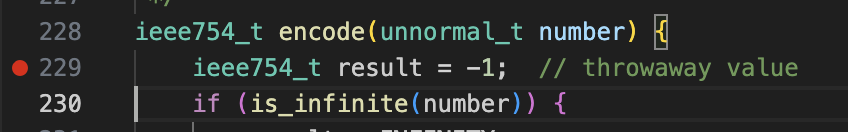
\includegraphics{rounding-images/setBreakpoint}
    }
    \checkoffitem{Launch \textit{floatlab} in the debugger, and use an input such as \texttt{\textbf{\textit{recode 1.1}}} \\
        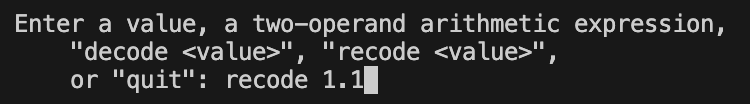
\includegraphics{rounding-images/enterTestValue}
    }
\end{description}

The driver code will parse the test value as an IEEE~754 single-precision value, so it will \textit{already} be rounded to fit in the available bits.
The trick is to re-introduce the bits that were rounded-off.

\begin{description}
    \checkoffitem{When the program reaches your breakpoint at the start of \function{encode()}, ``examine'' \lstinline{number.fraction}.}
    \checkoffitem{Instruct the debugger to change \lstinline{number.fraction}'s value.
        In VS~Code, this is done by right-clicking on the variable's name in the frame in which you're examining its value, and selecting ``Set Value''. \\
        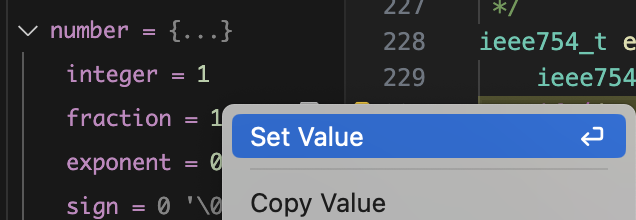
\includegraphics{rounding-images/selectSetValue}
    }
    \checkoffitem{Enter the 64-bit fraction for your test value in hexadecimal, such as \texttt{\textbf{\textit{recode 0x199999999999999A}}}
        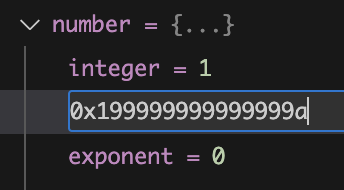
\includegraphics{rounding-images/newValueSet}
    }
    \checkoffitem{Instruct the debugger to continue. \\
        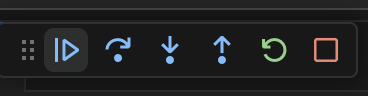
\includegraphics{rounding-images/selectContinue}
    }
    \checkoffitem{Compare the bit vector that your rounding code produced with the bit vector that it should have produced. \\
        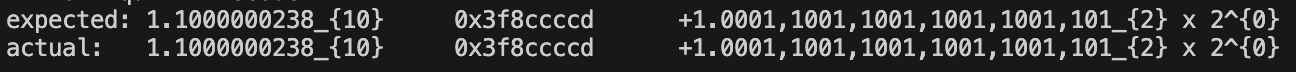
\includegraphics{rounding-images/results}
    }
\end{description}

\textit{Note: } Using this same technique to change \lstinline{number.exponent}, you can test your overflow-to-infinity and your underflow-to-zero code.

You may find these values useful for testing with the debugger:

\vspace{1cm}

\begin{tabular}[h]{ll}
    \textbf{Decimal Value}          & \textbf{64-bit fraction} \\
    \multicolumn{2}{c}{digit separators added for clarity; you won't be able to use them in the debugger} \\
    1.1                             & \texttt{0x1999'9999'9999'999A} \\
    1.3                             & \texttt{0x4CCC'CCCC'CCCC'CCCD} \\
    1.7                             & \texttt{0xB333'3333'3333'3333} \\
    1.9                             & \texttt{0xE666'6666'6666'6666} \\
    1.250'000'059'604'644'775'39    & \texttt{0x4000'0100'0000'0000} \\
    1.250'000'178'813'934'326'17    & \texttt{0x4000'0300'0000'0000}
\end{tabular}

\end{document}
